% Options for packages loaded elsewhere
\PassOptionsToPackage{unicode}{hyperref}
\PassOptionsToPackage{hyphens}{url}
%
\documentclass[
  12pt,
]{article}
\usepackage{amsmath,amssymb}
\usepackage{iftex}
\ifPDFTeX
  \usepackage[T1]{fontenc}
  \usepackage[utf8]{inputenc}
  \usepackage{textcomp} % provide euro and other symbols
\else % if luatex or xetex
  \usepackage{unicode-math} % this also loads fontspec
  \defaultfontfeatures{Scale=MatchLowercase}
  \defaultfontfeatures[\rmfamily]{Ligatures=TeX,Scale=1}
\fi
\usepackage{lmodern}
\ifPDFTeX\else
  % xetex/luatex font selection
\fi
% Use upquote if available, for straight quotes in verbatim environments
\IfFileExists{upquote.sty}{\usepackage{upquote}}{}
\IfFileExists{microtype.sty}{% use microtype if available
  \usepackage[]{microtype}
  \UseMicrotypeSet[protrusion]{basicmath} % disable protrusion for tt fonts
}{}
\makeatletter
\@ifundefined{KOMAClassName}{% if non-KOMA class
  \IfFileExists{parskip.sty}{%
    \usepackage{parskip}
  }{% else
    \setlength{\parindent}{0pt}
    \setlength{\parskip}{6pt plus 2pt minus 1pt}}
}{% if KOMA class
  \KOMAoptions{parskip=half}}
\makeatother
\usepackage{xcolor}
\usepackage[margin=1in]{geometry}
\usepackage{longtable,booktabs,array}
\usepackage{calc} % for calculating minipage widths
% Correct order of tables after \paragraph or \subparagraph
\usepackage{etoolbox}
\makeatletter
\patchcmd\longtable{\par}{\if@noskipsec\mbox{}\fi\par}{}{}
\makeatother
% Allow footnotes in longtable head/foot
\IfFileExists{footnotehyper.sty}{\usepackage{footnotehyper}}{\usepackage{footnote}}
\makesavenoteenv{longtable}
\usepackage{graphicx}
\makeatletter
\def\maxwidth{\ifdim\Gin@nat@width>\linewidth\linewidth\else\Gin@nat@width\fi}
\def\maxheight{\ifdim\Gin@nat@height>\textheight\textheight\else\Gin@nat@height\fi}
\makeatother
% Scale images if necessary, so that they will not overflow the page
% margins by default, and it is still possible to overwrite the defaults
% using explicit options in \includegraphics[width, height, ...]{}
\setkeys{Gin}{width=\maxwidth,height=\maxheight,keepaspectratio}
% Set default figure placement to htbp
\makeatletter
\def\fps@figure{htbp}
\makeatother
\setlength{\emergencystretch}{3em} % prevent overfull lines
\providecommand{\tightlist}{%
  \setlength{\itemsep}{0pt}\setlength{\parskip}{0pt}}
\setcounter{secnumdepth}{5}
\usepackage{setspace}
\onehalfspacing
\usepackage{booktabs}
\usepackage{longtable}
\usepackage{array}
\usepackage{multirow}
\usepackage{wrapfig}
\usepackage{float}
\usepackage{colortbl}
\usepackage{pdflscape}
\usepackage{tabu}
\usepackage{threeparttable}
\usepackage{threeparttablex}
\usepackage[normalem]{ulem}
\usepackage{makecell}
\usepackage{xcolor}
\ifLuaTeX
  \usepackage{selnolig}  % disable illegal ligatures
\fi
\IfFileExists{bookmark.sty}{\usepackage{bookmark}}{\usepackage{hyperref}}
\IfFileExists{xurl.sty}{\usepackage{xurl}}{} % add URL line breaks if available
\urlstyle{same}
\hypersetup{
  pdftitle={Project 1 Final report},
  pdfauthor={Shuai Zhu},
  hidelinks,
  pdfcreator={LaTeX via pandoc}}

\title{Project 1 Final report}
\author{Shuai Zhu}
\date{2024-10-05}

\begin{document}
\maketitle

\hypertarget{introduction}{%
\section{Introduction}\label{introduction}}

The data used in this analysis come from the ongoing Multicenter AIDS
Cohort Study (MACS), a prospective cohort study designed to understand
the natural and treated histories of HIV-1 infection in homosexual and
bisexual men across four major cities in the United States. This dataset
includes eight years of longitudinal data from 715 HIV-infected men,
capturing laboratory measurements, quality of life scores, demographic
information, and other health-related data collected after the
initiation of highly active antiretroviral therapy (HAART), which is the
standard treatment for patients with HIV.

The primary research question is to examine how treatment response, two
years after initiating HAART, differs between individuals who reported
hard drug use at baseline and those who did not. Four key measures of
treatment response are considered: viral load, CD4+ T cell counts, and
physical and mental quality of life scores.

\hypertarget{methods}{%
\section{Methods}\label{methods}}

\hypertarget{data-cleaning}{%
\subsection{Data cleaning}\label{data-cleaning}}

Baseline and two year measurement was filtered for further analysis
since the purpose of this project is find out how treatment response
differ two years after treatment. The data with BMI greater than 200 or
less than 0 was removed since it is impossible. The records with
complete case was used for further analysis and the number of
observations was reduced to 425. Furthermore, BMI was categorized to
four levels underweight (BMI \textless{} 18.5 kg/m2), healthy (BMI 18.5
- 24.9 kg/m2), overweight(BMI 24.9 - 30 kg/m2) and obese (BMI
\textgreater{} 30 kg/m2). Adherence was dichotomized into
\textgreater=95\% and \textless95\%. The education levels was collapsed
into three levels (High school or before, Some college, and Graduate or
Post-graduate).

\hypertarget{data-analysis}{%
\subsection{Data analysis}\label{data-analysis}}

Both frequentist and Bayesian approaches were employed to assess
differences in treatment response by baseline hard drug use. The four
key outcomes used to assess treatment response were viral load, CD4+ T
cell counts, and physical and mental quality of life scores (AGG\_PHYS
and AGG\_MENT). The objective was to model the impact of hard drug use,
adjusting for several covariates, including baseline treatment response,
BMI, age, education level, and adherence. Viral load, due to its skewed
distribution, was log-transformed to meet the assumption of normality.
For the frequentist approach, four multivariable linear regression
models were fitted, each predicting one of the treatment response
outcomes. The model assumptions---independence, linearity,
homoscedasticity, and normality---were carefully evaluated using
standard diagnostic tools. Independence was verified by inspecting the
structure of the data and residuals. Linearity was checked by assessing
the relationship between predictors and outcome variables using residual
plots. Homoscedasticity was evaluated using residuals vs.~fitted values
plots. Normality of residuals was tested through QQ-plots.

For Bayesian regression models, both non-informative and vague priors
were used. The non-informative priors of beta are distributed with mean
0 and standard deviation 10\^{}7. The vague priors of beta are
distributed with mean 0 and standard deviation 10\^{}6. The prior
distribution for the model error was set as a half-Cauchy distribution
with a scale parameter of 2.5. Bayesian inference was carried out using
Markov Chain Monte Carlo (MCMC) sampling. Each model was run with 4 MCMC
chains, with each chain consisting of 2,000 iterations, including a
1,000 iteration burn-in period to ensure convergence. The posterior
distributions for all model parameters were summarized, and credible
intervals were used to quantify uncertainty in the estimates.

For the frequentist models, standard metrics such as p-values and
confidence intervals were used to assess the significance and effect
sizes of the predictors. For the Bayesian models, the convergence of
MCMC chains was assessed through trace plots. Posterior means and 95\%
credible intervals were reported for each parameter to provide a full
picture of the uncertainty around the estimates.

R version 4.4.4 was used for all models.

\hypertarget{result}{%
\section{Result}\label{result}}

The percentage of missing data is visualized in Figure 1, where it is
evident that approximately 30\% of the data is missing for the four
outcome measurements of treatment response at year 2 and education
level. Viral load, CD4+ T cell count at baseline, and BMI level had a
smaller amount of missing data, ranging from 3.4\% to 5.9\%. In
contrast, physical and mental quality of life at baseline, age, and
adherence had almost no missing data. After excluding participants with
any missing values, 425 participants were retained for analysis, which
constitutes 58\% of the total sample. Among the participants with
complete cases, 35 (8.2\%) identified as hard drug users. These details
are summarized in Table 1.

The coefficients for hard drug use from both the frequentist approach
and the Bayesian approach (with vague priors) are presented in Table 2.
Both the 95\% confidence interval (frequentist) and the 95\% credible
interval (Bayesian) are reported to account for uncertainty in the
estimates. While Table 3 contains the coefficients and credible
intervals from the Bayesian approach using noninformative priors, the
estimates from the Bayesian approach with vague priors are closer to the
frequentist estimates. Therefore, the interpretation focuses on the
results from the frequentist approach and the Bayesian approach with
vague priors, without including the noninformative priors in the
following discussion.

\hypertarget{frequentist}{%
\subsection{Frequentist}\label{frequentist}}

After adjusting for baseline log viral load, age, BMI, education levels,
and adherence, the frequentist multivariable linear regression model
suggests that patients who identified as hard drug users at baseline had
0.96 times the viral load compared to those who did not identify as hard
drug users at baseline (95\% CI: (0.39, 2.39), p value = 0.9367). This
indicates that, on average, hard drug users had a slightly lower viral
load compared to non-drug users.

After adjusting for baseline CD4+ T cell counts, age, BMI, education
levels, and adherence, the frequentist multivariable linear regression
model suggests that patients who identified as hard drug users at
baseline had 186.284 lower CD4+ T cell counts compared to those who did
not identify as hard drug users at baseline with the confidence interval
suggesting that the true difference could range from a reduction of 124
to 249 CD4+ T cell(p value \textless{} 0.05).

After adjusting for baseline physical quality of life score, age, BMI,
education levels, and adherence, the frequentist multivariable linear
regression model suggests that patients who identified as hard drug
users at baseline had an average 3.32-point lower physical quality of
life score compared to non-drug users (95\% CI: -6.02, -0.62). The
confidence interval indicates that the true difference in physical
quality of life score could range from a reduction of 6.02 to 0.62
points, and since the p-value is less than 0.05, this result is
statistically significant, indicating a meaningful negative association
between hard drug use and physical quality of life.

After adjusting for baseline physical quality of life score, age, BMI,
education levels, and adherence, the frequentist multivariable linear
regression model suggests that patients who identified as hard drug
users at baseline had an average 1.17-point lower physical quality of
life score compared to non-drug users (95\% CI: -4.60, -2.25). The
confidence interval indicates that the true difference in physical
quality of life score could range from a reduction of 4.60 to 2.25
points, and since the p-value is less than 0.05, this result is
statistically significant. This suggests a meaningful negative
association between hard drug use and physical quality of life.

\hypertarget{bayesian}{%
\subsection{Bayesian}\label{bayesian}}

After adjusting for baseline log viral load, age, BMI, education levels,
and adherence, the Bayesian multivariable linear regression model using
vague priors suggests that patients who identified as hard drug users at
baseline had 0.96 times the viral load compared to those who did not
identify as hard drug users at baseline (95\% credible interval: 0.40,
2.34). This indicates that, on average, hard drug users had a slightly
lower viral load compared to non-drug users, although the wide credible
interval suggests considerable uncertainty, with the possibility that
the true effect could range from a substantial reduction to a potential
increase in viral load.

After adjusting for baseline CD4+ T cell count, age, BMI, education
levels, and adherence, the Bayesian multivariable linear regression
model using vague priors suggests that patients who identified as hard
drug users at baseline had an average 186.05 lower CD4+ T cell count
compared to those who did not identify as hard drug users at baseline
(95\% credible interval: -247.84, -123.01). This result indicates a
significant reduction in CD4+ T cell count among hard drug users, with
the credible interval suggesting that the true reduction could range
from 123 to 248 cells, reflecting a meaningful negative impact of hard
drug use on CD4+ T cell levels.

After adjusting for baseline physical quality of life score, age, BMI,
education levels, and adherence, the Bayesian multivariable linear
regression model using vague priors suggests that patients who
identified as hard drug users at baseline had an average 3.31-point
lower physical quality of life score compared to those who did not
identify as hard drug users at baseline (95\% credible interval: -6.07,
-0.61). This result indicates a significant reduction in physical
quality of life among hard drug users, with the credible interval
suggesting that the true reduction could range from 0.61 to 6.07 points,
reflecting a meaningful negative association between hard drug use and
physical quality of life.

After adjusting for baseline mental quality of life score, age, BMI,
education levels, and adherence, the Bayesian multivariable linear
regression model using noninformative priors suggests that patients who
identified as hard drug users at baseline had an average 1.18-point
lower mental quality of life score compared to those who did not
identify as hard drug users at baseline (95\% credible interval: -4.53,
2.24). This result suggests a potential reduction in mental quality of
life among hard drug users, but the wide credible interval, which
crosses zero, indicates uncertainty about the direction and significance
of the effect, meaning the true impact could range from a substantial
reduction to a potential increase in mental quality of life.

\hypertarget{conclusion}{%
\section{Conclusion}\label{conclusion}}

According to the results from both the frequentist approach and the
Bayesian approach with vague priors, there is no evidence of a
significant difference in viral load or mental quality of life scores
between patients with different hard drug use statuses. Similarly, there
is no evidence of a difference in CD4+ T cell counts or physical quality
of life scores between hard drug users and non-users. Overall, the
results from both the frequentist and Bayesian approaches with vague
priors are consistent and yield similar conclusions.

One limitation of this study is the small proportion of participants who
reported hard drug use at baseline (only 8.2\%). This low percentage
reduces the power of the analysis and may hinder the ability to detect
subtle effects. Collecting more data, particularly from hard drug users,
would improve the precision of the results and provide a stronger basis
for drawing conclusions about the impact of hard drug use on treatment
outcomes.

\newpage
\begin{table}
\centering
\caption{\label{tab:unnamed-chunk-2}Summary of outcomes and predictors stratified by hard drugs}
\centering
\fontsize{10}{12}\selectfont
\begin{tabular}[t]{llll}
\toprule
  & Hard drugs use & No hard drugs use & Overall\\
\midrule
 & (N=35) & (N=390) & (N=425)\\
\addlinespace[0.3em]
\multicolumn{4}{l}{\textbf{VLOAD\_year0}}\\
\hspace{1em}Mean (SD) & 204000 (450000) & 1010000 (12100000) & 940000 (11600000)\\
\hspace{1em}Median [Min, Max] & 29300 [739, 2520000] & 33300 [9.00, 191000000] & 32600 [9.00, 191000000]\\
\addlinespace[0.3em]
\multicolumn{4}{l}{\textbf{VLOAD\_year2}}\\
\hspace{1em}Mean (SD) & 36500 (120000) & 6060 (42400) & 8560 (53700)\\
\hspace{1em}Median [Min, Max] & 42.0 [0.740, 424000] & 31.0 [0.247, 711000] & 31.0 [0.247, 711000]\\
\addlinespace[0.3em]
\multicolumn{4}{l}{\textbf{LEU3N\_year0}}\\
\hspace{1em}Mean (SD) & 361 (204) & 377 (197) & 376 (197)\\
\hspace{1em}Median [Min, Max] & 453 [10.9, 650] & 361 [12.4, 1220] & 361 [10.9, 1220]\\
\addlinespace[0.3em]
\multicolumn{4}{l}{\textbf{LEU3N\_year2}}\\
\hspace{1em}Mean (SD) & 372 (252) & 565 (258) & 549 (263)\\
\hspace{1em}Median [Min, Max] & 357 [60.0, 971] & 544 [39.5, 1730] & 529 [39.5, 1730]\\
\addlinespace[0.3em]
\multicolumn{4}{l}{\textbf{AGG\_PHYS\_year0}}\\
\hspace{1em}Mean (SD) & 48.8 (6.86) & 51.5 (8.67) & 51.3 (8.56)\\
\hspace{1em}Median [Min, Max] & 46.7 [31.4, 62.9] & 53.7 [22.4, 69.0] & 53.5 [22.4, 69.0]\\
\addlinespace[0.3em]
\multicolumn{4}{l}{\textbf{AGG\_PHYS\_year2}}\\
\hspace{1em}Mean (SD) & 44.4 (12.1) & 50.0 (9.94) & 49.5 (10.2)\\
\hspace{1em}Median [Min, Max] & 45.5 [18.2, 63.9] & 53.3 [14.8, 68.9] & 53.2 [14.8, 68.9]\\
\addlinespace[0.3em]
\multicolumn{4}{l}{\textbf{AGG\_MENT\_year0}}\\
\hspace{1em}Mean (SD) & 42.6 (11.3) & 44.9 (13.9) & 44.7 (13.7)\\
\hspace{1em}Median [Min, Max] & 45.1 [22.9, 59.6] & 49.3 [7.23, 66.0] & 48.9 [7.23, 66.0]\\
\addlinespace[0.3em]
\multicolumn{4}{l}{\textbf{AGG\_MENT\_year2}}\\
\hspace{1em}Mean (SD) & 46.2 (14.2) & 47.7 (11.6) & 47.6 (11.8)\\
\hspace{1em}Median [Min, Max] & 49.6 [21.3, 65.3] & 51.2 [10.5, 66.7] & 51.2 [10.5, 66.7]\\
\addlinespace[0.3em]
\multicolumn{4}{l}{\textbf{Age}}\\
\hspace{1em}Mean (SD) & 44.2 (9.43) & 43.0 (8.82) & 43.1 (8.86)\\
\hspace{1em}Median [Min, Max] & 47.0 [29.0, 61.0] & 43.0 [20.0, 73.0] & 43.0 [20.0, 73.0]\\
\addlinespace[0.3em]
\multicolumn{4}{l}{\textbf{BMI}}\\
\hspace{1em}Healthy & 25 (71.4\%) & 192 (49.2\%) & 217 (51.1\%)\\
\hspace{1em}Obsese & 2 (5.7\%) & 47 (12.1\%) & 49 (11.5\%)\\
\hspace{1em}Overweight & 7 (20.0\%) & 138 (35.4\%) & 145 (34.1\%)\\
\hspace{1em}Underweight & 1 (2.9\%) & 13 (3.3\%) & 14 (3.3\%)\\
\addlinespace[0.3em]
\multicolumn{4}{l}{\textbf{Adh}}\\
\hspace{1em}Mean (SD) & 1.00 (0) & 0.897 (0.304) & 0.906 (0.292)\\
\hspace{1em}Median [Min, Max] & 1.00 [1.00, 1.00] & 1.00 [0, 1.00] & 1.00 [0, 1.00]\\
\addlinespace[0.3em]
\multicolumn{4}{l}{\textbf{Edu}}\\
\hspace{1em}Graduate, Post Graduate & 9 (25.7\%) & 81 (20.8\%) & 90 (21.2\%)\\
\hspace{1em}High school & 12 (34.3\%) & 80 (20.5\%) & 92 (21.6\%)\\
\hspace{1em}some college & 14 (40.0\%) & 229 (58.7\%) & 243 (57.2\%)\\
\bottomrule
\end{tabular}
\end{table}

\begin{longtable}[]{@{}
  >{\raggedright\arraybackslash}p{(\columnwidth - 12\tabcolsep) * \real{0.2083}}
  >{\raggedleft\arraybackslash}p{(\columnwidth - 12\tabcolsep) * \real{0.1667}}
  >{\raggedleft\arraybackslash}p{(\columnwidth - 12\tabcolsep) * \real{0.1250}}
  >{\raggedleft\arraybackslash}p{(\columnwidth - 12\tabcolsep) * \real{0.1250}}
  >{\raggedleft\arraybackslash}p{(\columnwidth - 12\tabcolsep) * \real{0.1250}}
  >{\raggedleft\arraybackslash}p{(\columnwidth - 12\tabcolsep) * \real{0.1250}}
  >{\raggedleft\arraybackslash}p{(\columnwidth - 12\tabcolsep) * \real{0.1250}}@{}}
\caption{Comparions of estimate and 95\% confident intervals and credit
intervals between Frequentist and Bayesian approach}\tabularnewline
\toprule\noalign{}
\begin{minipage}[b]{\linewidth}\raggedright
\end{minipage} & \begin{minipage}[b]{\linewidth}\raggedleft
Frequentist
\end{minipage} & \begin{minipage}[b]{\linewidth}\raggedleft
2.5\%
\end{minipage} & \begin{minipage}[b]{\linewidth}\raggedleft
97.5\%
\end{minipage} & \begin{minipage}[b]{\linewidth}\raggedleft
Vague
\end{minipage} & \begin{minipage}[b]{\linewidth}\raggedleft
2.5\%
\end{minipage} & \begin{minipage}[b]{\linewidth}\raggedleft
97.5\%
\end{minipage} \\
\midrule\noalign{}
\endfirsthead
\toprule\noalign{}
\begin{minipage}[b]{\linewidth}\raggedright
\end{minipage} & \begin{minipage}[b]{\linewidth}\raggedleft
Frequentist
\end{minipage} & \begin{minipage}[b]{\linewidth}\raggedleft
2.5\%
\end{minipage} & \begin{minipage}[b]{\linewidth}\raggedleft
97.5\%
\end{minipage} & \begin{minipage}[b]{\linewidth}\raggedleft
Vague
\end{minipage} & \begin{minipage}[b]{\linewidth}\raggedleft
2.5\%
\end{minipage} & \begin{minipage}[b]{\linewidth}\raggedleft
97.5\%
\end{minipage} \\
\midrule\noalign{}
\endhead
\bottomrule\noalign{}
\endlastfoot
Log Viral Load & -0.037 & -0.946 & 0.873 & -0.035 & -0.916 & 0.852 \\
CD4+ Count & -186.284 & -248.508 & -124.060 & -186.052 & -247.837 &
-123.013 \\
Physical score & -3.319 & -6.015 & -0.623 & -3.307 & -6.069 & -0.610 \\
Mental score & -1.172 & -4.598 & 2.253 & -1.183 & -4.526 & 2.244 \\
\end{longtable}

\begin{longtable}[]{@{}lrrr@{}}
\caption{Estimatae and 95\% Credit interval of Bayesian approach with
noninformative priors}\tabularnewline
\toprule\noalign{}
& Estimate & 2.5\% & 97.5\% \\
\midrule\noalign{}
\endfirsthead
\toprule\noalign{}
& Estimate & 2.5\% & 97.5\% \\
\midrule\noalign{}
\endhead
\bottomrule\noalign{}
\endlastfoot
Log Viral Load & -0.045358 & -0.9430382 & 0.8793678 \\
CD4+ Cell Count & -185.667304 & -248.4468299 & -124.5246236 \\
Physical score & -3.321138 & -6.0445899 & -0.6430269 \\
Mental score & -1.199944 & -4.6906949 & 2.3279289 \\
\end{longtable}

\begin{figure}
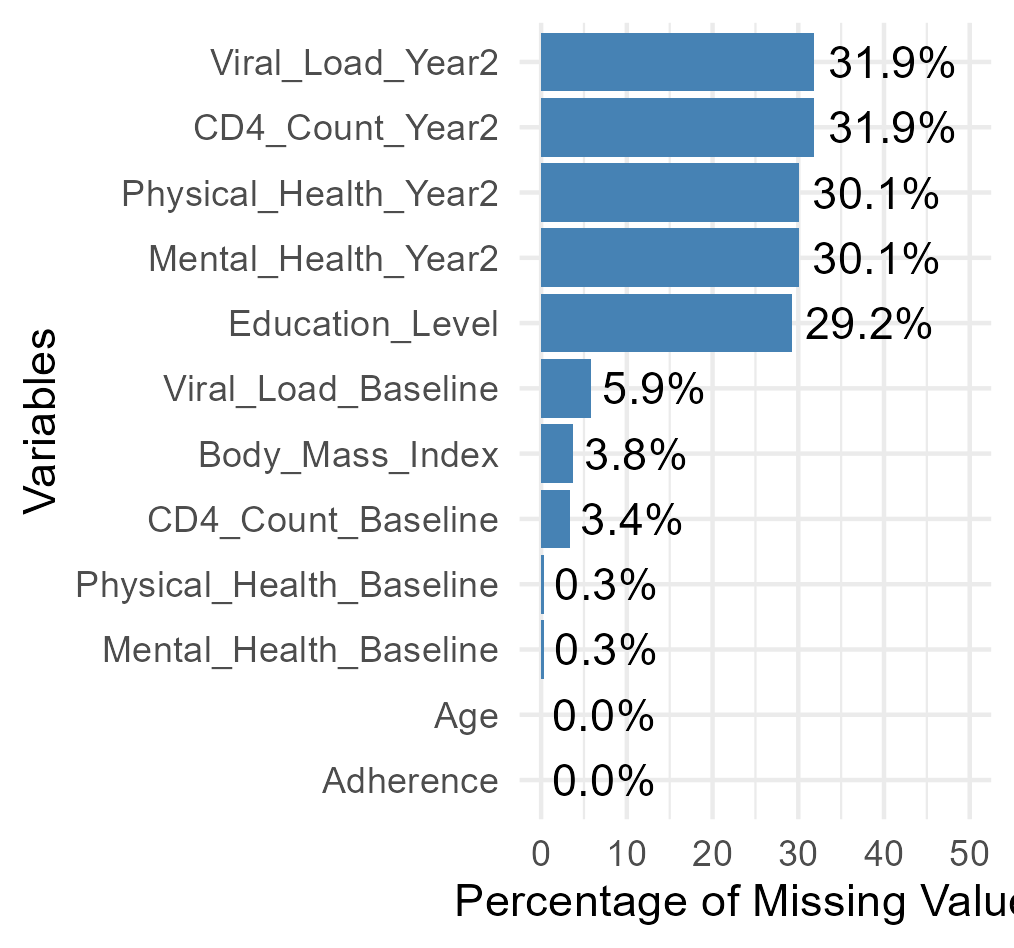
\includegraphics[width=14.08in]{../DataProcessed/missing visulization} \caption{Percentage of Missing Data by Variable}\label{fig:unnamed-chunk-4}
\end{figure}

\end{document}
